%(BEGIN_QUESTION)
% Copyright 2015, Tony R. Kuphaldt, released under the Creative Commons Attribution License (v 1.0)
% This means you may do almost anything with this work of mine, so long as you give me proper credit

Skisser ledningskobling slik at denne datainnsamlingsmodulen (DAQ) kan indikere lysintensitet på inngangskanal {\tt IN 2} (dvs. mindre lys skal gi sterkere positiv avlesning i DAQ). Legg gjerne til ekstra komponenter du mener er nødvendige.

\vskip 50pt

$$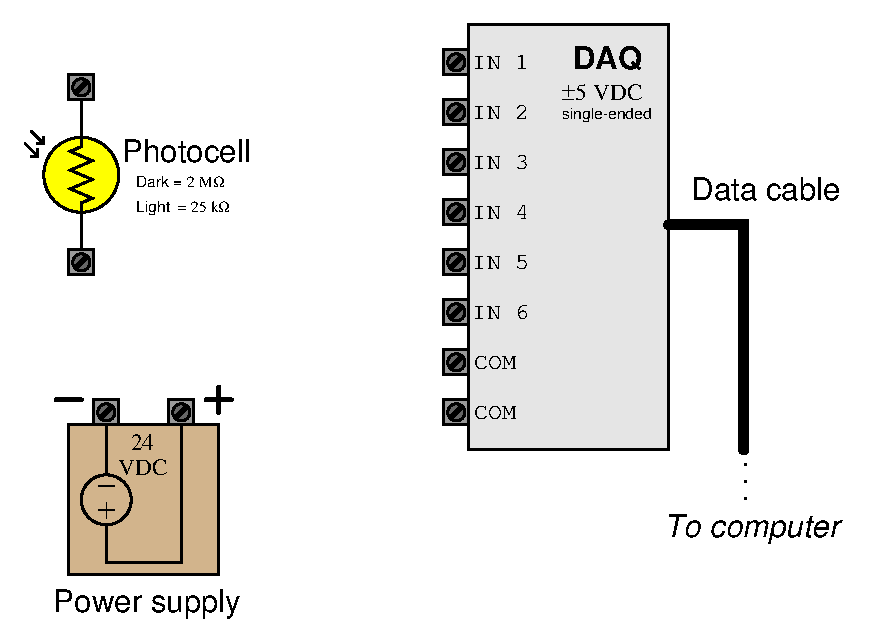
\includegraphics[width=15.5cm]{i00383x01.eps}$$

\underbar{file i00383}
%(END_QUESTION)





%(BEGIN_ANSWER)

Enhver løsning der DAQ kanal \#2 måler mer positiv spenning når fotocellemotstanden øker (fotocellen mørklegges), er riktig:

$$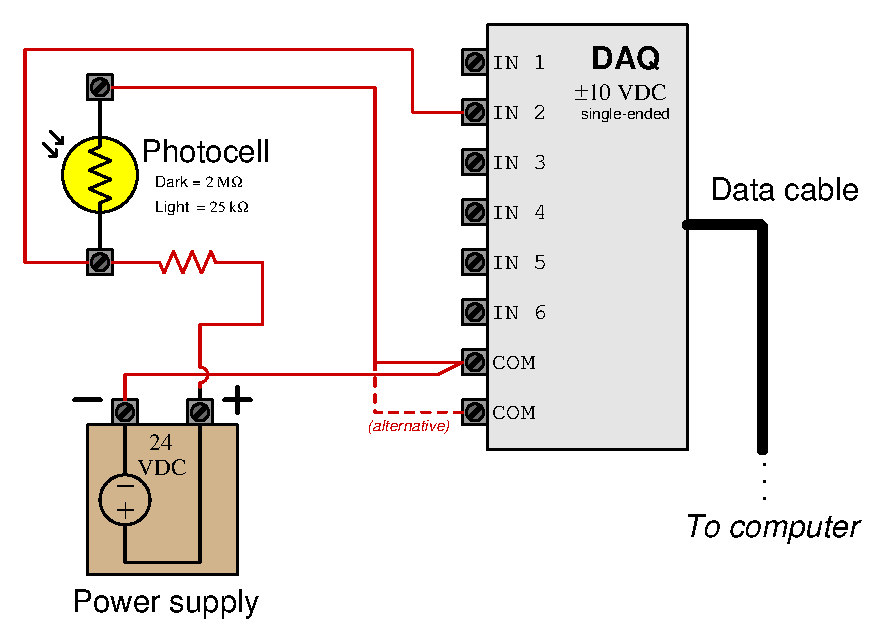
\includegraphics[width=15.5cm]{i00383x02.eps}$$

%(END_ANSWER)





%(BEGIN_NOTES)

{\bf Denne oppgaven er ment for eksamen og ikke for arbeidsark!}.

%(END_NOTES)
